\chapter{Exemplos \LaTeX}
\label{cap-exemplos}

\explicacao{ATENÇÃO : Este capítulo e os seguintes demonstram como fazer no {\LaTeX} portanto devem ser lidos em conjunto com o código fonte desse documento}

% exemplo de como inserir uma referencia adicional no sumario (normalmente não utilizado em um trabalho acadêmico)
\addcontentsline{toc}{chapter}{Exemplos que devem ser lidos (mas esse tipo de indicação não vai em um trabalho acadêmico) :-)}

Esse capítulo tem exemplos de escrita utilizando o {\LaTeX}  utilizando \abnTeX, é muito simples escrever em \textbf{negrito}, \textit{itálico} \footnote{apesar de que nesse documento \mostraComandoLaTeX{textit} \mostraComandoLaTeX{emph} tem comportamento parecido é recomendável utilizar \mostraComandoLaTeX{textit} de forma genérica para itálico}, ....


Existem diversos tutoriais para uso de \LaTeX, se você está utilizando esse modelo não precisará se preocupar com muitos dos detalhes técnicos do \LaTeX \space e cuidar somente do seu texto.

Escolha seu editor : \url{https://en.wikipedia.org/wiki/Comparison\_of\_TeX\_editors}, apesar do overleaf sem bem prático, nem todas as funções estão disponíveis na versão gratuita e você pode instalar gratuitamente em seu computador um compilador \LaTeX \space e utilizar um sistema de controle de versão para gerenciar seu documento.


\section{Normas ABNT}

Esse documento modelo já resolve boa parte da padronização NBR 14.724:2011 \cite{NBR14724:2011} que deve ser seguida e inclusive alguns pontos que não são claros pelo modelo de padronização do \ac{ifsp}.

Leia os documentos do {\abnTeX} e do \ac{ifsp}:
\begin{itemize}
    \item \url{https://www.abntex.net.br/}
    
    \item \acs{faq} : \url{https://github.com/abntex/abntex2/wiki/FAQ}
    
    \item \url{http://mirror.unl.edu/ctan/macros/latex/contrib/abntex2/doc/abntex2.pdf}
    
    \item \waUrl{https://spo.ifsp.edu.br/biblioteca?id=184}
\end{itemize}

No \ac{ifsp} você pode acessar todas as normas \ac{abnt} sem custo, as informações estão disponíveis no endereço \waUrl{https://www.ifsp.edu.br/index.php/outras-noticias/52-reitoria/2329-alunos-e-servidores-do-ifsp-podem-acessar-abnt-via-web.html}.

Apesar de alguns elementos serem opcionais na \ac{abnt} eles foram definidos como obrigatórios (folha de rosto, resumo, lista de siglas, lista de ilustrações, glossário etc), nos trabalhos completos de projetos de informática do \ac{ifsp} campus São Paulo. Documentos menores como propostas de projeto, documento de \ac{poc} não necessitam desses elementos, mas alguns podem ser uteis para ajudar no estudo do {\LaTeX} em preparação para o documento final.

\begin{itemize}
    \item Logotipo da instituição, não é citado na \ac{abnt} nem no manual de normalização do \ac{ifsp}, mas aparece em uma imagem do documento de normalização, foi definido que não deve ser incluído na capa;
    
    \item Nome da instituição que é opcional na capa, deve ser utilizado;
    
\end{itemize}



\section{Detalhes textuais}

O documento é dividido em capítulos, e cada capítulo dividido em seções utilizando o \abnTeX \space você pode dividir seus documentos nos níveis de acordo com os comandos:

\begin{itemize}
    \item \mostraComandoLaTeX{chapter}  (1);
    
    \item \mostraComandoLaTeX{section} (1.1);
    
    \item \mostraComandoLaTeX{subsection} (1.1.1);
    
    \item \mostraComandoLaTeX{subsubsection} (1.1.1.1);
    
    \item \mostraComandoLaTeX{subsubsubsection} (1.1.1.1.1).
    
\end{itemize}

Tenha em mente que normalmente se utiliza no máximo o nível \mostraComandoLaTeX{subsection}.
Ao definir as divisões do seu trabalho utilizando as diretivas do \LaTeX, elas são automaticamente inseridas no sumário do documento.


\subsection{Caracteres Reservados e auxiliares}



Alguns caracteres são reservados no \LaTeX \space e por isso para utilizar esses caracteres é necessário utilizar uma forma diferenciada de escrita. É possível utilizar a macro \mostraComandoLaTeX{symbol} com o código \ac{ascii} do caracter desejado, veja no código fonte desse texto como utilizar corretamente esses itens.


\begin{itemize}
\item barra invertida : \textbackslash   \symbol{92}    $\backslash$;
\item til  :  \symbol{126} ;
\item cifrão : \$;
\item sublinhado, \textit{underscore}, \textit{underline} : \_;
\item \enquote{aspas} as macros \mostraComandoLaTeX{enquote} / \mostraComandoLaTeX{textquote} garantem o espaçamento correto, se utilizar diretamente as ASPAS o espaçamento é perdido;
% https://tex.stackexchange.com/questions/80395/no-space-after-closing-double-quote
\item marcadores : \cmark\ \xmark\ \circlemark\ \ding{100} \ - ver mais no \refanexo{pifont-quickref};
\item chaves : \} \{.
\end{itemize}

\subsection{Listas}

Em uma lista de itens cada item deve ser terminado por ponto e virgula, exceto o ultimo item que deve ter um ponto final.

\begin{itemize}
\item item 1;
\item item 2;
\item item ..;
\item item final.
\end{itemize}


\subsection{Citações / Referências}
\label{referencias}

Em um trabalho acadêmico você deve buscar referencias que servem de base para seus estudos, essas referencias devem ser confiáveis, normalmente artigos e livros são confiáveis pois passam por um processo de revisão por especialistas na área. É importante buscar as referencias primárias e não utilizar a informação escrita por outra pessoa (referencia secundária). As citações são definidas pela \citetitle{NBR10520:2002} e as referencias pela \citetitle{NBR6023:2018}, sendo interessante observar que a \citeonline{NBR6023:2018_alteracoes} fez uma resumo com algumas das mudanças ocorridas em 2018.


A \ac{abnt} define a citação da citação (\textit{apud}), mas sua utilização não deve ser feita exceto em casos onde o documento original não possa ser acessado de nenhuma forma. Atualmente a maioria dos documentos se encontra disponível de forma digital o que permite a busca das informações em suas fontes primárias de forma que o \textit{apud} não é bem visto. 

Não é indicada a utilização de sites como Wikipedia como fonte de informações pois a Wikipedia é uma referencia secundária, já que exige que seus artigos tenham referencias da informação, e com isso a utilização da Wikipedia cai no mesmo caso da utilização de \textit{apud} indicada anteriormente, já que é possível buscar a informação diretamente na fonte primária.

Quando for necessário citar sites deve ser utilizada a ferramenta \url{https://web.archive.org}, caso não exista uma referencia salva anteriormente basta salvar e utilizar. O uso dessa ferramenta muitas vezes ajuda também a determinar a data estimada de publicação de informação quando o site já foi salvo anteriormente e não possui data de publicação disponível.



Existem diversas formas de citação que devem ser escolhidas de acordo com o contexto do texto onde são utilizadas, observe os exemplos :

\begin{itemize}
    \item \mostraComandoLaTeX{cite} - utilizada normalmente em final de paragrafo: \newline
    \cite{UML:JACOBSON} | \cite{POWELL:2006} \\ 
        \cite{SCRUMGUIDE:2013} | \cite{urani1994} |\\
        \cite{ETAL5} | \cite{ETAL4}; 
    
    \explicacao{Se as duas ultimas referencias aparecem somente com um autor, você está compilando o documento com uma versão antiga do \mostraPacoteLaTeX{abntexcite}, o overleaf em 2021-07-06 estava desatualizado}
    \explicacao{ABNT 6023:2018 8.1.1.2 recomenda para utilizar TODOS autores sempre, mas permite utilizar et al, dependendo da versão do \mostraPacoteLaTeX{abntexcite} isso não está acontecendo corretamente}

    \item \mostraComandoLaTeX{citeonline}  - utilizada normalmente em textos como \enquote{(segundo|de acordo| com) ...}: \newline
    \citeonline{UML:JACOBSON} | \citeonline{POWELL:2006} \\
        \citeonline{SCRUMGUIDE:2013} | \citeonline{urani1994} \\
        \citeonline{ETAL5} | \citeonline{ETAL4};

    \item \mostraComandoLaTeX{citeauthoronline} - raramente utilizado, quando se deseja citar somente o autor: \newline
    \citeauthoronline{UML:JACOBSON}| \citeauthoronline{POWELL:2006} \\
        \citeauthoronline{SCRUMGUIDE:2013} | \citeauthoronline{urani1994} \\
        \citeauthoronline{ETAL5} | \citeauthoronline{ETAL4};

    \item \mostraComandoLaTeX{citeauthor} - muito pouco utilizado: \newline \citeauthor{UML:JACOBSON}| \citeauthor{POWELL:2006} \\
        \citeauthor{SCRUMGUIDE:2013}| \citeauthor{urani1994} \\
        \citeauthor{ETAL5} | \citeauthor{ETAL4};
    
    \explicacao{Se as duas ultimas referencias aparecem somente com um autor, você está compilando o documento com uma versão antiga do \mostraPacoteLaTeX{abntexcite}, o overleaf em 2021-07-06 estava desatualizado}

    \item \mostraComandoLaTeX{citetitle} - muito pouco utilizado: \newline
    \citetitle{UML:JACOBSON}|\citetitle{POWELL:2006} \\
        \citetitle{SCRUMGUIDE:2013}| \citetitle{urani1994} 
        
    \explicacao{O comando \mostraComandoLaTeX{citetitle} está disponível utilizando a biblioteca \mostraPacoteLaTeX{biblatex}}

\end{itemize}

A documentação do abntex2cite possui muitos exemplos de como utilizar corretamente cada formato de citação : \url{https://mirrors.ibiblio.org/CTAN/macros/latex/contrib/abntex2/doc/abntex2cite-alf.pdf}.

Cada formato de citação deve ser utilizado em um contexto especifico :
\begin{itemize}
    \item De acordo com \citeonline{SCRUMGUIDE:2013} .....;
    
    \item Fonte: \citeonline{SCRUMGUIDE:2013};
    
    \item sua explicação de um assunto baseado em uma referência \cite{SCRUMGUIDE:2013}.
    
\end{itemize}

ATENÇÃO : Alguns parâmetros de formatação foram alterados em 2018, mas não foram corrigidos ainda nos pacotes do \ac{abntex}, devem ser alterados manualmente ou utilizar as versões de desenvolvimento
\begin{itemize}
    \item \url{https://github.com/abntex/abntex2/issues/210}
    
    \item \url{https://github.com/abntex/biblatex-abnt/issues/42}
\end{itemize}

Os dados devem ser definidos corretamente nos arquivos \textquote{.bib} para a correta formatação no texto e na lista de referências.

Para autor com diversas publicações no mesmo ano : são geradas letras automaticamente pelo compilador de acordo com a ordem que são apresentadas na bibliografia, a letra não aparece na lista de referencias. \footnote{\url{https://github.com/abntex/biblatex-abnt/issues/20}}




\subsection{Abreviaturas / Siglas / Glossário}
\label{siglas-glossario}

Palavras que devem ser apresentadas no glossário devem ser citadas especificamente no texto utilizando os comandos de glossário como : \gls{tag}. Nesse modelo as definições de glossário devem ser feitas no arquivo \textbf{defs-glossario.tex}.

As abreviaturas nesse modelo devem ser feitas no arquivo \textbf{defs-siglas.tex}, tomando o cuidado de definir corretamente as siglas de outras línguas e as da língua portuguesa. Abreviaturas normalmente são referenciadas utilizando \mostraComandoLaTeX{ac}, mas podem ser referenciadas diretamente na versão reduzida \textquote{\acs{ifsp}} (\mostraComandoLaTeX{acs}) \space  
ou longa \textquote{\acl{ifsp}} (\mostraComandoLaTeX{acl}).

Na primeira vez que a sigla aparecer no texto o compilador {\LaTeX} mostra por extenso e a partir dai mostra somente a sigla:

\begin{itemize}
    \item \ac{se}
    
    \item \ac{se}
    
\end{itemize}

Quando uma sigla é utilizada em titulo de figura ela não deve aparecer por extenso. A maneira correta para que isso aconteça é utilizar a sigla com \mostraComandoLaTeX{acs} no titulo da figura como apresentado na \autoref{fig_sge1} pela sigla \ac{sge1}.

\begin{figure}[hb]
    \centering
	\caption{\label{fig_sge1}Exemplo de sigla em titulo de ilustração \acs{sge1}}
    \missingfigure[figwidth=6cm]{Exemplo para uso de sigla em titulo \ldots}	
	\fonte{Os autores.}
\end{figure}



Lembre que o {\LaTeX} tem vários passos de compilação, sempre que alterar as chamadas de siglas / referencias é recomendável uma compilação completa do documento.








\subsection{Elementos não textuais / Ilustrações}
\label{elementos-nao-textuais}

Elementos não textuais são aqueles que auxiliam o entendimento, não podem ficar \enquote{jogados} no texto, devem ser citados, cada elemento deve ser identificado por um \mostraComandoLaTeX{label} único que permite a sua referencia, no texto utilizando \mostraComandoLaTeX{ref} ou \mostraComandoLaTeX{autoref}, esses elementos quando definidos corretamente também são inseridos nas listas presentes antes do sumário.

Cuidado com o artigo \textbf{O/A} antes da Figura, Tabela ou Quadro referenciado, deve ser compatível com o tipo da ilustração.

Lembre que o \LaTeX \  vai posicionar os elementos  da melhor maneira possível dentro do documento, sempre faça as referencias utilizando os comandos específicos, nunca utiliza \enquote{acima}, \enquote{"baixo}, \enquote{a seguir}, etc... 

O posicionamento desses elementos é feito pelas rotinas do pacote float, leia a documentação em  \url{http://linorg.usp.br/CTAN/macros/latex/contrib/float/float.pdf}. É recomendável utilizar as opções de posicionamento \textbf{htb}, a opção \textbf{H} deverá ser utilizada somente como ultima alternativa de posicionamento e em alguns casos a utilização de \mostraComandoLaTeX{FloatBarrier} pode também melhorar o resultado se utilizada com cuidado.

Lembre que se houver uma grande distancia entre a ilustração no documento \ac{pdf} e sua definição original no documento isso significa que existe muito pouco texto em seu documento e isso não oferece muitas opções para o {\LaTeX} organizar as ilustrações. Você precisa nesse caso melhorar a descrição textual das ilustrações.


Para casos onde existe uma grande distancia entre a ilustração e o ponto de referencia no texto esse modelo possui macros \mostraComandoLaTeX{autorefwithpage} e \mostraComandoLaTeX{autorefwithpagedistance} a primeira sempre indica página onde a ilustração foi colocada e a segunda somente se a ilustração estiver mais distante que o número de páginas indicado como parâmetro, Ex. \autorefwithpage{fig_logo_A3}. Isso deve ser utilizado somente quando existe mais de uma referencia para mesma ilustração e não para deixar a ilustração distante de uma única referencia.

O titulo da ilustração deve ser apresentado sempre no topo (conforme \citetitle{NBR14724:2011}, era na parte inferior na  \citetitle{NBR14724:2005}), e a fonte deve ficar na parte inferior \cite{NBR14724:2011}. A norma não possui um exemplo direto do uso das fontes e é possível encontrar exemplos com e sem ponto final nas fontes das ilustrações. Considerando a utilização de ponto no manual do \ac{ibge} nesse modelo foi escolhido utilizar o ponto final na fonte das ilustrações.





% ---
\subsection{QR-Code}
% ---
\index{qr-code}
A utilização de códigos \ac{qr} facilita o acesso de endereços da internet a partir de dispositivos móveis com câmera.
As figuras \ref{qr-url-1} e \ref{qr-url-2} demonstram dois exemplos de endereços apresentados com essa tecnologia.


Para facilitar a utilização dos códigos \ac{qr}, deve-se tomar cuidado para não deixa-los alinhados na vertical pois dificulta a seleção a partir da câmera no dispositivo móvel.

Um exemplo para utilização de mais códigos de barra pode ser visto em : \urlmodelo.

Atenção, alguns compiladores podem ter problemas em utilizar a biblioteca \textbf{pstricks} necessária para gerar QR-Codes, no sharelatex em 2017-05 a compilação ocorre perfeitamente utilizando a opção de compilador "XeLatex", ele é mais lento que outras opções.


\begin{figure}
\begin{pspicture}(25mm,25mm)
\psbarcode{\urlmodelosimples}{eclevel=H width=1.0 height=1.0}{qrcode}
\end{pspicture}
\caption{\label{qr-url-1}QR-Code - URL Documento exemplo}
\legend{\urlmodelo}
\fonte{Os Autores}
\end{figure}



% colocando figura qrcode na direita para facilitar o uso da camera deixando cada qrcode em um alinhamento diferente
% se deixar os dois qrcodes um em cima do outro dificulta acessar o desejado
\begin{figure}
\begin{flushright}
\begin{pspicture}(25mm,25mm)
\psbarcode{https://github.com/ivanfmartinez/latexlib/tree/master/ifsp}{eclevel=H width=1.0 height=1.0}{qrcode}
\end{pspicture}
\caption{\label{qr-url-2}QR-Code - Classes IFSP GitHub}
\legend{\url{https://github.com/ivanfmartinez/latexlib/tree/master/ifsp}}
\fonte{Os Autores}
\end{flushright}

\end{figure}


\subsection{Organizando pendências}

Durante o desenvolvimento de um trabalho escrito é normal que alguns elementos sejam gerados posteriormente, mas é importante se organizar para não esquecer de fazer os ajustes necessários. Para isso recomendo a utilização do pacote \textbf{todonotes} que oferece diversos recursos para gerar lembretes das pendencias. O manual do \textbf{todonotes} está disponível no \autoref{manual-todonotes}\footnote{observe que existe um erro nesse documento, já que a referencia deveria ser Anexo e aparece como Apêndice,  existe um \textit{bug} no abntex2 ao referenciar anexos, para fazer corretamente veja \url{https://github.com/abntex/abntex2/issues/76} e utilize \mostraComandoLaTeX{refanexo} que está disponível nesse modelo.}.

É possível fazer anotações de pendencias inclusive indicando as pessoas responsáveis por elas, % nao mover o todo pois foi feito no meio do paragrafo exatamente para demonstrar um possível problema de formato
\todo[inline,author=Pessoa1]{fazer revisão das imagens do texto} e para facilitar a visualização criar imagens que funcionam como marcadores para figuras que serão incluídas posteriormente.

Cuidado ao utilizar as anotações \textit{inline} pois o texto ficara quebrado, como no paragrafo anterior.


\begin{figure}[htb]
    \centering
	\caption{\label{fig_todo1}Imagem que ainda não foi gerada}
	\missingfigure[figwidth=10cm]{você está atrasado pois ainda não criou esta figura}
	\fonte{dados do Projeto.}
\end{figure}



\subsection{Tabelas e Quadros}
\label{tabelas-e-quadros}
Quadros e Tabelas são informações tabulares, mas Tabelas tem como objetivo apresentar números. A ‘norma’ 14724 \cite[3.32]{NBR14724:2011} define a Tabela como sendo uma \enquote{forma não discursiva de apresentar informações das quais o dado numérico se destaca como informação central} e que devem seguir padronização do \ac{ibge}  \cite[5.9]{NBR14724:2011}. O \ac{ibge} padronizou a apresentações de dados tabulares em 1993 \cite{tabular-ibge}.

Informações adicionais sobre o de tabelas no {\LaTeX} podem ser obtidas em  \url{https://en.wikibooks.org/wiki/LaTeX/Tables}.

Antes de utilizar \index{longtable}\textbf{longtable} procure reorganizar o seu layout ou quebrar manualmente em múltiplos quadros / tabelas, pois isso ainda facilita a compreensão pelo leitor.

% https://biblioteca.ibge.gov.br/visualizacao/livros/liv23907.pdf

\index{quadros}O \autoref{quadro-exemplo} é um exemplo de dados tabulares gerados em 
\LaTeX.



\begin{quadro}[htb]
\centering
\ABNTEXfontereduzida
\caption[Níveis de investigação]{Níveis de investigação}
\label{quadro-exemplo}
\begin{tabular}{|p{2.6cm}|p{6.0cm}|p{2.25cm}|p{3.40cm}|}
  \hline
   \thead{Nível de\\Investigação} & \thead{Insumos}  & \thead{Sistemas de\\ Investigação}  & \thead{Produtos}  \\
    \hline
    Meta-nível & Filosofia\index{filosofia} da Ciência  & Epistemologia &
    Paradigma  \\
    \hline
    Nível do objeto & Paradigmas do metanível e evidências do nível inferior &
    Ciência  & Teorias e modelos \\
    \hline
    Nível inferior & Modelos e métodos do nível do objeto e problemas do nível inferior & Prática & Solução de problemas  \\
   \hline
\end{tabular}
\fonte{O Autor.}
\end{quadro}



\index{tabelas}Já a \autoref{tab-exemplo} foi criada conforme o padrão \citeonline{tabular-ibge} requerido pelas normas da \ac{abnt} para documentos técnicos e acadêmicos. Observe que não existem bordas laterais e nem linhas separadoras em uma Tabela e as colunas numéricas tem alinhamento à direita. 

\begin{table}[htb]
\centering
\caption{Métricas de desenvolvimento}
\label{tab-exemplo}
\begin{tabular}{p{2.6cm}rrr}
    \hline
   \thead{Item} & \thead{Janeiro}  & \thead{Fevereiro}  & \thead{Março}  \\
    \hline
    Classes & 2  & 10 & 20  \\
    Linhas & 100  & 250 & 543 \\
    \hline
\end{tabular}
\fonte{Os autores.}
\end{table}

\def\equationautorefname~#1\null{%
  Equação~(#1)\null
}


Para facilitar a criação de tabelas e quadros existem algumas ferramentas como o Tables Generator \url{http://www.tablesgenerator.com/latex_tables} que permite a criação de forma visual gerando o código \LaTeX\ correspondente. E o site \url{https://www.latex-tables.com/} permite converter planilhas em código \LaTeX.


\index{equação}\index{Pitágoras}A \autoref{eq-pythagoras} demonstra que também é possível escrever equações diretamente em \LaTeX

\begin{equation}\label{eq-pythagoras}
a^2+b^2=c^2\,.
\end{equation}






% ---
\subsection{Figuras}
\label{sec_figuras}
% ---

\index{figuras}Figuras podem ser criadas diretamente em \LaTeX,
como o exemplo da \autoref{fig_circulo}, ou inseridas a partir de arquivos externos como a \autoref{fig_logo}, que é o Logotipo do \ac{ifsp}. \index{logotipo}

% Aqui foi utilizada uma figura unica para demostrar a diferença de qualidade entr e vetorizado e não vetorizado pois fica mais simples, já que cada leitor pode ver esse documento em monitores com diferentes qualidades...
As figuras externas devem possuir boa qualidade e preferencialmente serem vetorizadas para se obter o melhor resultado. A \autoref{fig:nao_vetorizado_e_vetorizado} apresenta duas versões de uma mesma imagem demonstrando a variação de qualidade que pode acontecer quando não for utilizada a versão vetorizada, quando a figura possui elementos textuais pode até inviabilizar a leitura. As Figuras \ref{fig:uml_dia_nao_vetorizado_jpeg}, \ref{fig:uml_dia_vetorizado_eps} e \ref{fig:uml_dia_vetorizado_svg} foram reduzidas propositalmente no documento para demonstrar a diferença entre os formatos de arquivo. A diferença fica mais perceptível quando o documento é impresso ou quando existem textos pequenos e é necessário fazer zoom para visualização.

Procure criar suas imagens e diagramas pensando em utilizar impressão em preto-e-branco ou escala de cinza. Isto é importante, principalmente quando se pretende publicar o trabalho, uma vez que a maioria das publicações são somente em preto-e-branco. Outro benefício é o custo de impressão, normalmente menor para páginas preto-e-branco em relação a páginas coloridas.

Para diagramas em \ac{uml} o PlantUML pode ser utilizado para gerar código {\LaTeX} como exemplo na  \autoref{diagramauml}.


Se não houver a possibilidade de utilização de uma imagem vetorizada e existem diversos detalhes utilize \ac{png} em vez de \gls{jpg} ou outros formatos de menor qualidade, observe as diferenças nos exemplos apresentados em :  \waUrlTitle{https://tex.stackexchange.com/questions/136087/selecting-best-file-extension-for-graphics-figures-pictures}{Selecting best file extension for graphics figures pictures}.


\begin{figure}[htb]
	\caption{\label{fig_circulo}A delimitação do espaço}
	\begin{center}
	    \setlength{\unitlength}{5cm}
		\begin{picture}(1,1)
		\put(0,0){\line(0,1){1}}
		\put(0,0){\line(1,0){1}}
		\put(0,0){\line(1,1){1}}
		\put(0,0){\line(1,2){.5}}
		\put(0,0){\line(1,3){.3333}}
		\put(0,0){\line(1,4){.25}}
		\put(0,0){\line(1,5){.2}}
		\put(0,0){\line(1,6){.1667}}
		\put(0,0){\line(2,1){1}}
		\put(0,0){\line(2,3){.6667}}
		\put(0,0){\line(2,5){.4}}
		\put(0,0){\line(3,1){1}}
		\put(0,0){\line(3,2){1}}
		\put(0,0){\line(3,4){.75}}
		\put(0,0){\line(3,5){.6}}
		\put(0,0){\line(4,1){1}}
		\put(0,0){\line(4,3){1}}
		\put(0,0){\line(4,5){.8}}
		\put(0,0){\line(5,1){1}}
		\put(0,0){\line(5,2){1}}
		\put(0,0){\line(5,3){1}}
		\put(0,0){\line(5,4){1}}
		\put(0,0){\line(5,6){.8333}}
		\put(0,0){\line(6,1){1}}
		\put(0,0){\line(6,5){1}}
		\end{picture}
	\end{center}
	\fonte{Modelo Canônico ABNTeX2.}
\end{figure}


\begin{figure}[htb]
    \centering
	\caption{\label{fig_logo}Logotipo \ac{ifsp}}
	
\includegraphics{\ifspprefixo/logo-02.jpg}
	\fonte{\ac{ifsp}.}
\end{figure}

\begin{figure}
    \centering
    \caption{Exemplo de imagem não vetorizada e vetorizada}
    \label{fig:nao_vetorizado_e_vetorizado}
	
\includegraphics[width=0.95\textwidth]{erros/exemploVetorizacao.png}
    \fonte{\citeonline{vetorizacao}.}
\end{figure}
    

% Essas imagens foram reduzidas na apresentação para demonstrar o efeito da alteração de escala em imagens não vetorizadas
\begin{figure}
    \centering
    \caption{Exemplo de diagrama - salvo em imagem não vetorizada - JPEG}
    \label{fig:uml_dia_nao_vetorizado_jpeg}
	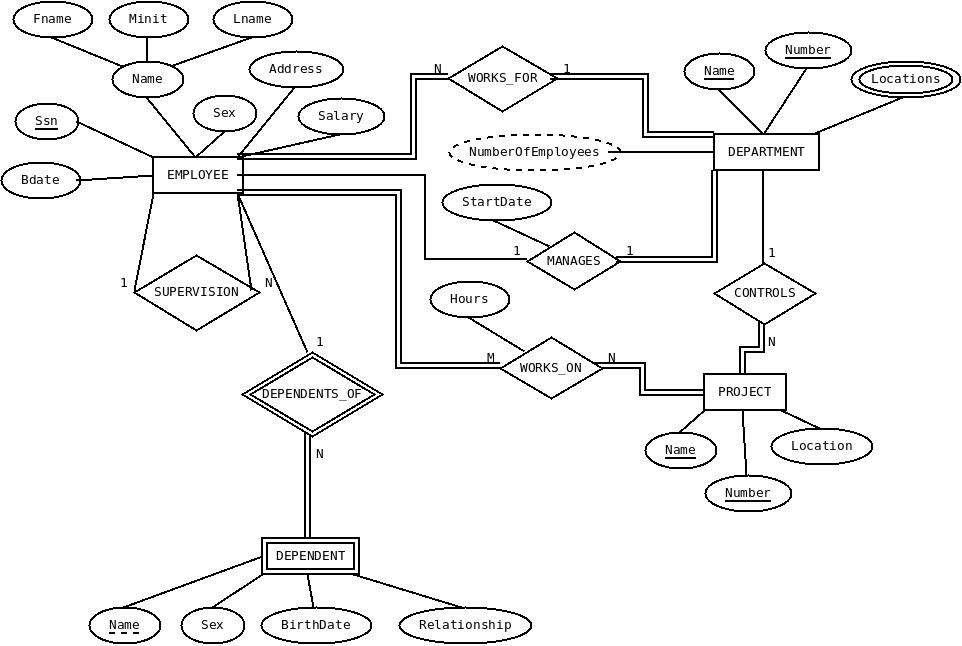
\includegraphics[width=0.6\textwidth]{exemplos/diagramas/ER.jpeg}
    \fonte{Indicar autor original.}
\end{figure}


\begin{figure}
    \centering
    \caption{Exemplo de diagrama - salvo imagem vetorizada - EPS}
    \label{fig:uml_dia_vetorizado_eps}
	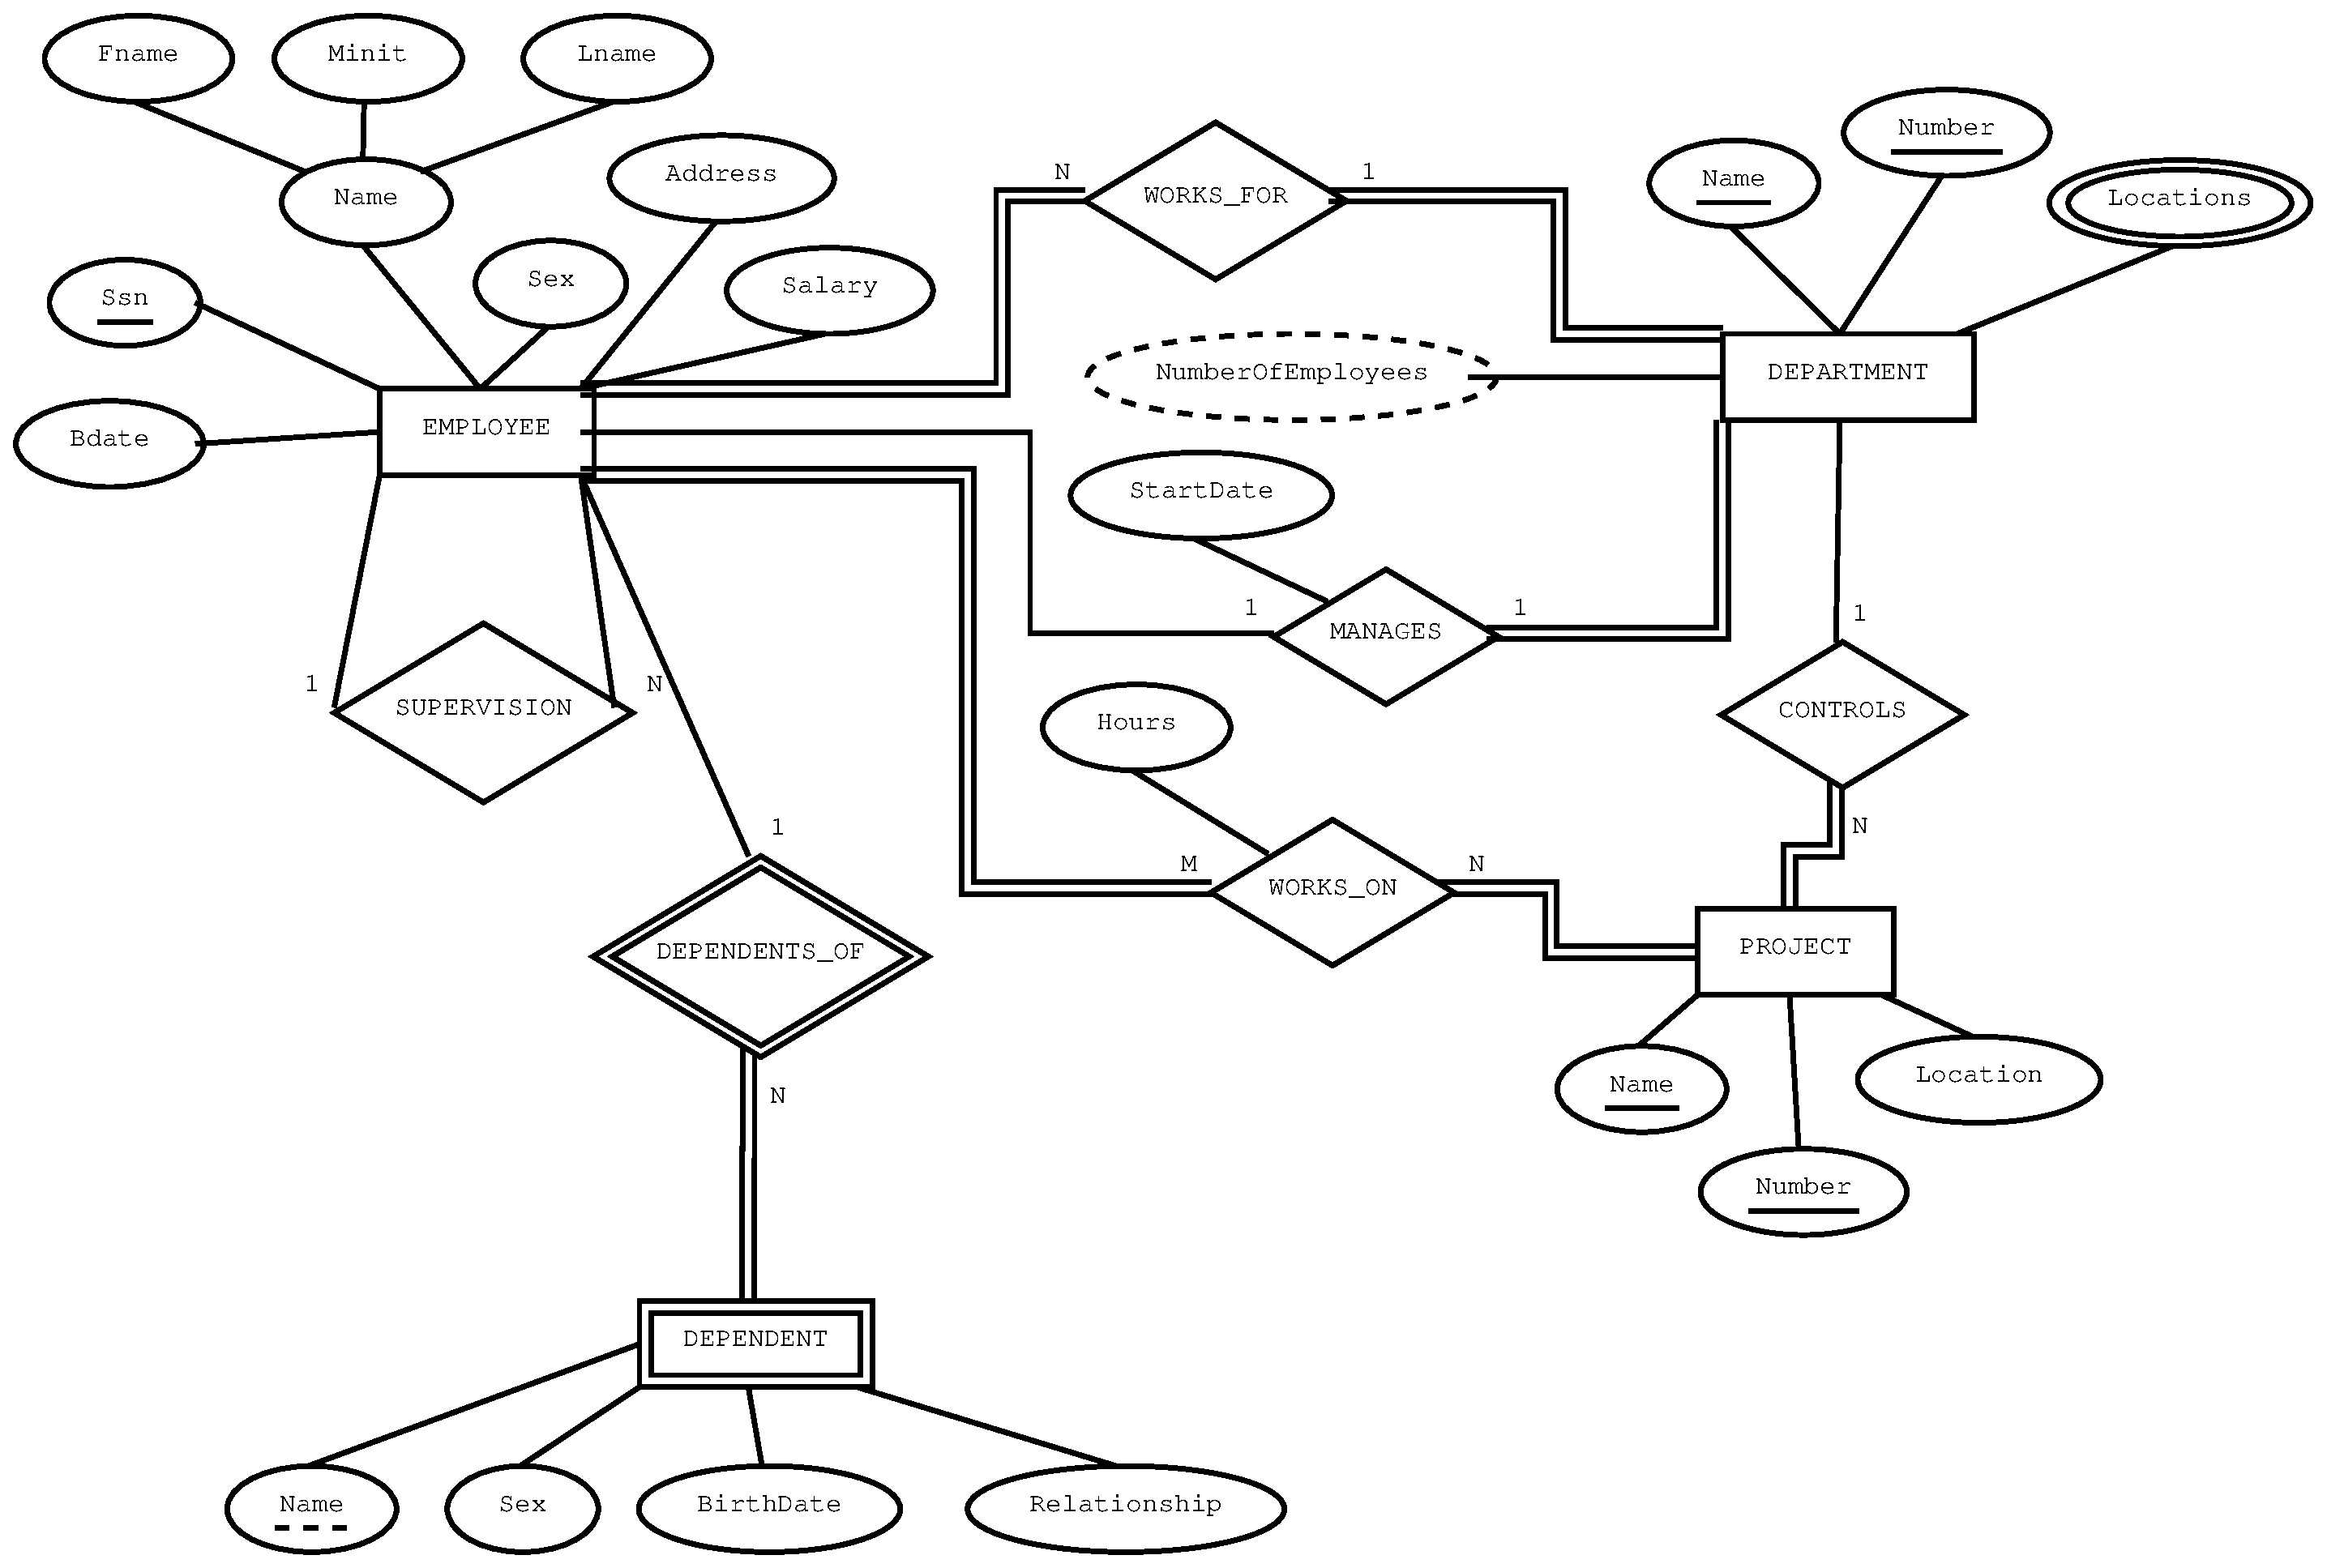
\includegraphics[width=0.6\textwidth]{exemplos/diagramas/ER.eps}
    \fonte{Indicar autor original.}
\end{figure}

\begin{figure}
    \centering
    \caption{Exemplo de diagrama - salvo imagem vetorizada - SVG}
    \label{fig:uml_dia_vetorizado_svg}
    \includesvg[inkscapelatex=false,width=0.6\textwidth]{exemplos/diagramas/ER.svg}
    \fonte{Indicar autor original.}
\end{figure}



% generated by Plantuml 7997beta
\definecolor{plantucolor0000}{RGB}{254,254,206}
\definecolor{plantucolor0001}{RGB}{168,0,54}
\definecolor{plantucolor0002}{RGB}{173,209,178}
\definecolor{plantucolor0003}{RGB}{0,0,0}
\definecolor{plantucolor0004}{RGB}{0,0,255}

\begin{figure}[htb]
    \centering
    \caption{\label{diagramauml}Exemplo de Diagrama UML gerado a partir do PlantUML}
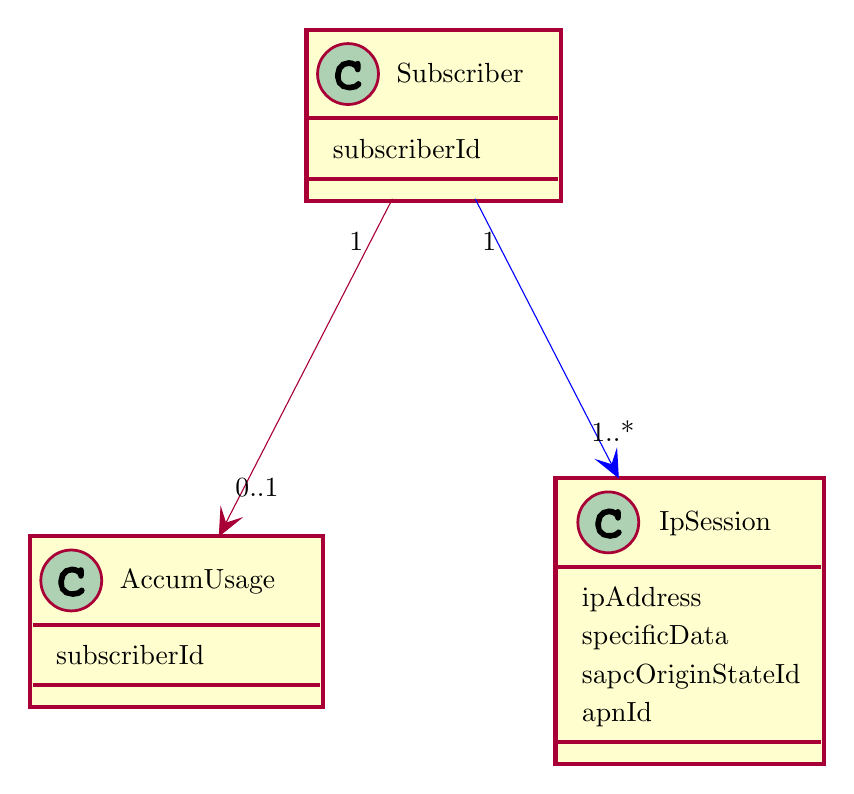
\begin{tikzpicture}[yscale=-1]
\draw[color=plantucolor0001,fill=plantucolor0000,line width=1.5pt] (131pt,29pt) rectangle (223pt,90.8359pt);
\draw[color=plantucolor0001,fill=plantucolor0002,line width=1.0pt] (146pt,45pt) ellipse (11pt and 11pt);
\draw[color=black,fill=black] (148.7656pt,40.875pt) ..controls (148.9219pt,40.6563pt) .. (149.1094pt,40.5469pt) ..controls (149.2969pt,40.4375pt) .. (149.5156pt,40.4375pt) ..controls (149.8906pt,40.4375pt) .. (150.125pt,40.6953pt) ..controls (150.3594pt,40.9531pt) .. (150.3594pt,41.5625pt) -- (150.3594pt,43.0156pt) ..controls (150.3594pt,43.625pt) .. (150.125pt,43.8906pt) ..controls (149.8906pt,44.1563pt) .. (149.5156pt,44.1563pt) ..controls (149.1719pt,44.1563pt) .. (148.9688pt,43.9531pt) ..controls (148.7656pt,43.7656pt) .. (148.6563pt,43.25pt) ..controls (148.6094pt,42.8906pt) .. (148.4219pt,42.7031pt) ..controls (148.0938pt,42.3281pt) .. (147.4844pt,42.1094pt) ..controls (146.875pt,41.8906pt) .. (146.25pt,41.8906pt) ..controls (145.4844pt,41.8906pt) .. (144.8516pt,42.2188pt) ..controls (144.2188pt,42.5469pt) .. (143.7266pt,43.2969pt) ..controls (143.2344pt,44.0469pt) .. (143.2344pt,45.0781pt) -- (143.2344pt,46.1719pt) ..controls (143.2344pt,47.4063pt) .. (144.125pt,48.2266pt) ..controls (145.0156pt,49.0469pt) .. (146.6094pt,49.0469pt) ..controls (147.5469pt,49.0469pt) .. (148.2031pt,48.7969pt) ..controls (148.5938pt,48.6406pt) .. (149.0156pt,48.2031pt) ..controls (149.2813pt,47.9375pt) .. (149.4297pt,47.8594pt) ..controls (149.5781pt,47.7813pt) .. (149.7813pt,47.7813pt) ..controls (150.1094pt,47.7813pt) .. (150.3672pt,48.0391pt) ..controls (150.625pt,48.2969pt) .. (150.625pt,48.6406pt) ..controls (150.625pt,48.9844pt) .. (150.2813pt,49.3906pt) ..controls (149.7813pt,49.9688pt) .. (148.9844pt,50.2969pt) ..controls (147.9063pt,50.75pt) .. (146.6094pt,50.75pt) ..controls (145.0938pt,50.75pt) .. (143.8906pt,50.125pt) ..controls (142.9063pt,49.625pt) .. (142.2188pt,48.5547pt) ..controls (141.5313pt,47.4844pt) .. (141.5313pt,46.2031pt) -- (141.5313pt,45.0469pt) ..controls (141.5313pt,43.7188pt) .. (142.1484pt,42.5703pt) ..controls (142.7656pt,41.4219pt) .. (143.8594pt,40.8047pt) ..controls (144.9531pt,40.1875pt) .. (146.1875pt,40.1875pt) ..controls (146.9219pt,40.1875pt) .. (147.5703pt,40.3516pt) ..controls (148.2188pt,40.5156pt) .. (148.7656pt,40.875pt);
\node at (160pt,37.4531pt)[below right]{Subscriber};
\draw[color=plantucolor0001,line width=1.5pt] (132pt,61pt) -- (222pt,61pt);
\node at (137pt,65pt)[below right]{subscriberId};
\draw[color=plantucolor0001,line width=1.5pt] (132pt,82.8359pt) -- (222pt,82.8359pt);
\draw[color=plantucolor0001,fill=plantucolor0000,line width=1.5pt] (31pt,212pt) rectangle (137pt,273.8359pt);
\draw[color=plantucolor0001,fill=plantucolor0002,line width=1.0pt] (46pt,228pt) ellipse (11pt and 11pt);
\draw[color=black,fill=black] (48.7656pt,223.875pt) ..controls (48.9219pt,223.6563pt) .. (49.1094pt,223.5469pt) ..controls (49.2969pt,223.4375pt) .. (49.5156pt,223.4375pt) ..controls (49.8906pt,223.4375pt) .. (50.125pt,223.6953pt) ..controls (50.3594pt,223.9531pt) .. (50.3594pt,224.5625pt) -- (50.3594pt,226.0156pt) ..controls (50.3594pt,226.625pt) .. (50.125pt,226.8906pt) ..controls (49.8906pt,227.1563pt) .. (49.5156pt,227.1563pt) ..controls (49.1719pt,227.1563pt) .. (48.9688pt,226.9531pt) ..controls (48.7656pt,226.7656pt) .. (48.6563pt,226.25pt) ..controls (48.6094pt,225.8906pt) .. (48.4219pt,225.7031pt) ..controls (48.0938pt,225.3281pt) .. (47.4844pt,225.1094pt) ..controls (46.875pt,224.8906pt) .. (46.25pt,224.8906pt) ..controls (45.4844pt,224.8906pt) .. (44.8516pt,225.2188pt) ..controls (44.2188pt,225.5469pt) .. (43.7266pt,226.2969pt) ..controls (43.2344pt,227.0469pt) .. (43.2344pt,228.0781pt) -- (43.2344pt,229.1719pt) ..controls (43.2344pt,230.4063pt) .. (44.125pt,231.2266pt) ..controls (45.0156pt,232.0469pt) .. (46.6094pt,232.0469pt) ..controls (47.5469pt,232.0469pt) .. (48.2031pt,231.7969pt) ..controls (48.5938pt,231.6406pt) .. (49.0156pt,231.2031pt) ..controls (49.2813pt,230.9375pt) .. (49.4297pt,230.8594pt) ..controls (49.5781pt,230.7813pt) .. (49.7813pt,230.7813pt) ..controls (50.1094pt,230.7813pt) .. (50.3672pt,231.0391pt) ..controls (50.625pt,231.2969pt) .. (50.625pt,231.6406pt) ..controls (50.625pt,231.9844pt) .. (50.2813pt,232.3906pt) ..controls (49.7813pt,232.9688pt) .. (48.9844pt,233.2969pt) ..controls (47.9063pt,233.75pt) .. (46.6094pt,233.75pt) ..controls (45.0938pt,233.75pt) .. (43.8906pt,233.125pt) ..controls (42.9063pt,232.625pt) .. (42.2188pt,231.5547pt) ..controls (41.5313pt,230.4844pt) .. (41.5313pt,229.2031pt) -- (41.5313pt,228.0469pt) ..controls (41.5313pt,226.7188pt) .. (42.1484pt,225.5703pt) ..controls (42.7656pt,224.4219pt) .. (43.8594pt,223.8047pt) ..controls (44.9531pt,223.1875pt) .. (46.1875pt,223.1875pt) ..controls (46.9219pt,223.1875pt) .. (47.5703pt,223.3516pt) ..controls (48.2188pt,223.5156pt) .. (48.7656pt,223.875pt);
\node at (60pt,220.4531pt)[below right]{AccumUsage};
\draw[color=plantucolor0001,line width=1.5pt] (32pt,244pt) -- (136pt,244pt);
\node at (37pt,248pt)[below right]{subscriberId};
\draw[color=plantucolor0001,line width=1.5pt] (32pt,265.8359pt) -- (136pt,265.8359pt);
\draw[color=plantucolor0001,fill=plantucolor0000,line width=1.5pt] (221pt,191pt) rectangle (318pt,294.3438pt);
\draw[color=plantucolor0001,fill=plantucolor0002,line width=1.0pt] (240.05pt,207pt) ellipse (11pt and 11pt);
\draw[color=black,fill=black] (242.8156pt,202.875pt) ..controls (242.9719pt,202.6563pt) .. (243.1594pt,202.5469pt) ..controls (243.3469pt,202.4375pt) .. (243.5656pt,202.4375pt) ..controls (243.9406pt,202.4375pt) .. (244.175pt,202.6953pt) ..controls (244.4094pt,202.9531pt) .. (244.4094pt,203.5625pt) -- (244.4094pt,205.0156pt) ..controls (244.4094pt,205.625pt) .. (244.175pt,205.8906pt) ..controls (243.9406pt,206.1563pt) .. (243.5656pt,206.1563pt) ..controls (243.2219pt,206.1563pt) .. (243.0188pt,205.9531pt) ..controls (242.8156pt,205.7656pt) .. (242.7063pt,205.25pt) ..controls (242.6594pt,204.8906pt) .. (242.4719pt,204.7031pt) ..controls (242.1438pt,204.3281pt) .. (241.5344pt,204.1094pt) ..controls (240.925pt,203.8906pt) .. (240.3pt,203.8906pt) ..controls (239.5344pt,203.8906pt) .. (238.9016pt,204.2188pt) ..controls (238.2688pt,204.5469pt) .. (237.7766pt,205.2969pt) ..controls (237.2844pt,206.0469pt) .. (237.2844pt,207.0781pt) -- (237.2844pt,208.1719pt) ..controls (237.2844pt,209.4063pt) .. (238.175pt,210.2266pt) ..controls (239.0656pt,211.0469pt) .. (240.6594pt,211.0469pt) ..controls (241.5969pt,211.0469pt) .. (242.2531pt,210.7969pt) ..controls (242.6438pt,210.6406pt) .. (243.0656pt,210.2031pt) ..controls (243.3313pt,209.9375pt) .. (243.4797pt,209.8594pt) ..controls (243.6281pt,209.7813pt) .. (243.8313pt,209.7813pt) ..controls (244.1594pt,209.7813pt) .. (244.4172pt,210.0391pt) ..controls (244.675pt,210.2969pt) .. (244.675pt,210.6406pt) ..controls (244.675pt,210.9844pt) .. (244.3313pt,211.3906pt) ..controls (243.8313pt,211.9688pt) .. (243.0344pt,212.2969pt) ..controls (241.9563pt,212.75pt) .. (240.6594pt,212.75pt) ..controls (239.1438pt,212.75pt) .. (237.9406pt,212.125pt) ..controls (236.9563pt,211.625pt) .. (236.2688pt,210.5547pt) ..controls (235.5813pt,209.4844pt) .. (235.5813pt,208.2031pt) -- (235.5813pt,207.0469pt) ..controls (235.5813pt,205.7188pt) .. (236.1984pt,204.5703pt) ..controls (236.8156pt,203.4219pt) .. (237.9094pt,202.8047pt) ..controls (239.0031pt,202.1875pt) .. (240.2375pt,202.1875pt) ..controls (240.9719pt,202.1875pt) .. (241.6203pt,202.3516pt) ..controls (242.2688pt,202.5156pt) .. (242.8156pt,202.875pt);
\node at (254.95pt,199.4531pt)[below right]{IpSession};
\draw[color=plantucolor0001,line width=1.5pt] (222pt,223pt) -- (317pt,223pt);
\node at (227pt,227pt)[below right]{ipAddress};
\node at (227pt,240.8359pt)[below right]{specificData};
\node at (227pt,254.6719pt)[below right]{sapcOriginStateId};
\node at (227pt,268.5078pt)[below right]{apnId};
\draw[color=plantucolor0001,line width=1.5pt] (222pt,286.3438pt) -- (317pt,286.3438pt);
\draw[color=plantucolor0004] (191.942pt,90.081pt) ..controls (205.204pt,115.893pt) and (224.952pt,154.325pt) .. (241.265pt,186.076pt);
\draw[color=plantucolor0004,fill=plantucolor0004] (243.646pt,190.709pt) -- (243.0894pt,180.8759pt) -- (241.3604pt,186.262pt) -- (235.9742pt,184.5329pt) -- (243.646pt,190.709pt) -- cycle;
\node at (191.0584pt,98.9168pt)[below right]{1};
\node at (230.3817pt,166.6703pt)[below right]{1..*};
\draw[color=plantucolor0001] (162.058pt,90.081pt) ..controls (145.645pt,122.023pt) and (119.302pt,173.295pt) .. (101.824pt,207.31pt);
\draw[color=plantucolor0001,fill=plantucolor0001] (99.5252pt,211.784pt) -- (107.1969pt,205.6078pt) -- (101.8108pt,207.337pt) -- (100.0816pt,201.9509pt) -- (99.5252pt,211.784pt) -- cycle;
\node at (143.0082pt,98.7264pt)[below right]{1};
\node at (101.801pt,187.522pt)[below right]{0..1};
\end{tikzpicture}
	\legend{Fonte: Exemplos PlantUML.}
\end{figure}

A \autoref{fig_diag_virado} exemplifica como utilizar uma imagem em formato paisagem (página inteira). Obs: Utilizamos propositalmente uma imagem não vetorizada de forma a ilustrar o procedimento e também para apresentar que a qualidade não fica boa o suficiente para leitura. Uma versão vetorizada dessa figura teria qualidade melhor.


% observe que a imagem a seguir teve que ser ajustada para caber corretamente na página
% por não ser uma imagem vetorizada a qualidade não é a melhor possivel
\begin{sidewaysfigure}[htb]
    \centering
	\caption{\label{fig_diag_virado}Diagrama Virado - Exemplo}
	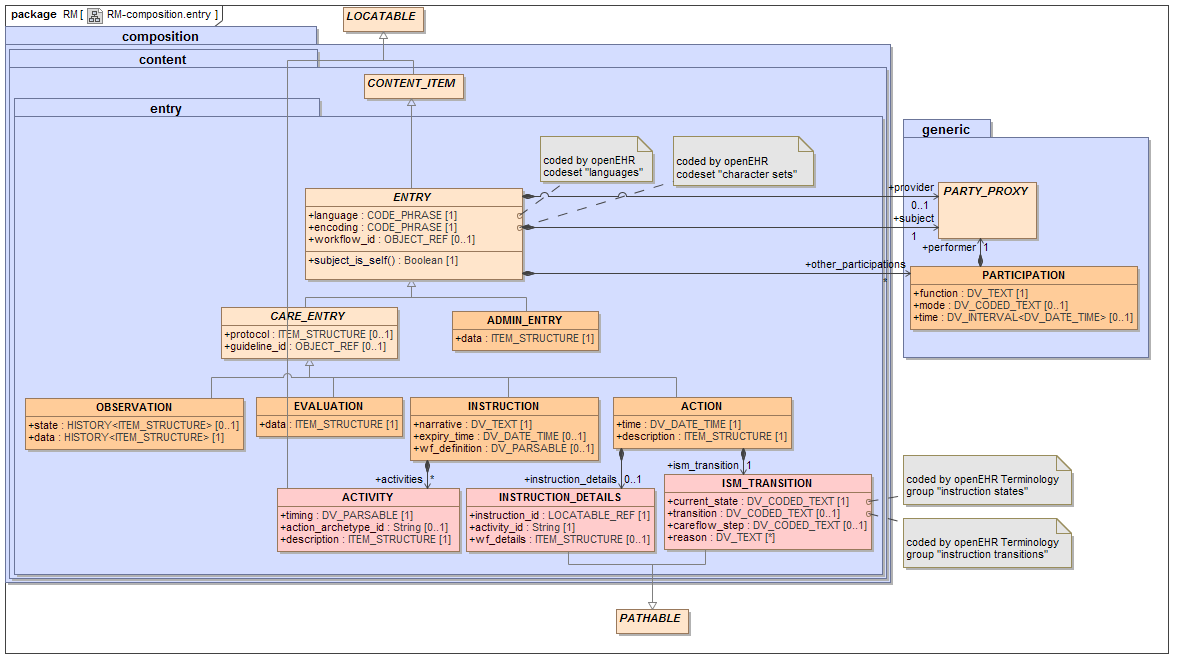
\includegraphics[width=0.9\textwidth]{exemplos/exemplo_diag_horizontal.png}
	\fonte{\citeonline{openehrCompositionEntry}.}
\end{sidewaysfigure}


\subsection{Impressão em folhas formato A3}

A página seguinte em A3 permite a impressão de diagramas grandes que não podem ser visualizados facilmente em folha padrão A4. Lembre que algumas impressoras podem ter problemas com isso, então selecione somente as páginas A4 ao imprimir e depois imprima separadamente a página A3.

A \autoref{fig_logo_A3} utiliza a mesma imagem da \autoref{fig_logo} e foi ampliada para demonstrar a essa possibilidade de impressão de grandes imagens em A3.

Observe que o código de exemplo vai gerar uma quebra de página no local onde for definida a página A3, por isso não deve ser utilizado entre textos para evitar grandes espaços em branco.

Folhas impressas em A3 ou tamanhos maiores devem ser dobradas seguindo o padrão definido pela \ac{abnt}. 


Cuidado ao utilizar folhas A3 em um documento impresso em frente e verso pois a numeração das páginas seguintes pode ser impressa de forma incorreta (posição do número na página). Uma alternativa para esta situação é manter todas páginas impressas em A3 no último apêndice, fazendo as referencias corretas durante o texto.



 \afterpage{%
 \begin{PAGINA-A3}

 \begin{figure}[p]
     \centering%
 	\caption{\label{fig_logo_A3}Logotipo \acs{ifsp} em página A3}
     \fcolorbox{red}{yellow}{ 
\includegraphics[height=\textheight,width=\textwidth,keepaspectratio]{\ifspprefixo/logo-02.jpg}}%
 	\legend{Com borda para demonstrar os limites}
   \fonte{citar o autor da Figura(xxx).}
 \end{figure}

 \end{PAGINA-A3}
 }

